\chapter{Contexte de l'étude}
\label{chap:contexte}

\section{Le corridor Dakar–Bamako : enjeux logistiques et économiques}
\label{sec:corridor}

\subsection{Géographie et importance stratégique du corridor}
Le Mali se caractérise par sa situation géographique de pays enclavé, dépourvu de tout accès direct à la mer. Cette configuration structurelle impose à son économie une dépendance critique vis-à-vis des infrastructures de transport des pays côtiers de la zone ouest-africaine. Dans ce contexte, le Port Autonome de Dakar s'impose comme le principal débouché et la porte d’accès maritime naturelle pour les flux d'importation et d'exportation maliens. 

Le corridor routier reliant Dakar à Bamako se déploie sur une distance d'environ 1~400 kilomètres. Cet axe représente une artère vitale par laquelle transite jusqu'à 80 \% du commerce global du Mali. L'approvisionnement en produits de première nécessité ainsi que l'acheminement des intrants industriels et agricoles reposent de manière prépondérante sur la continuité opérationnelle de cet axe géoéconomique majeur, comme le soulignent les travaux de Byiers et Rosengren \cite{byiersActeursInteretsLong2022} (cf. figure~\ref{fig:corridor_dakar_bamako}).
\begin{figure}[H]
  \centering
  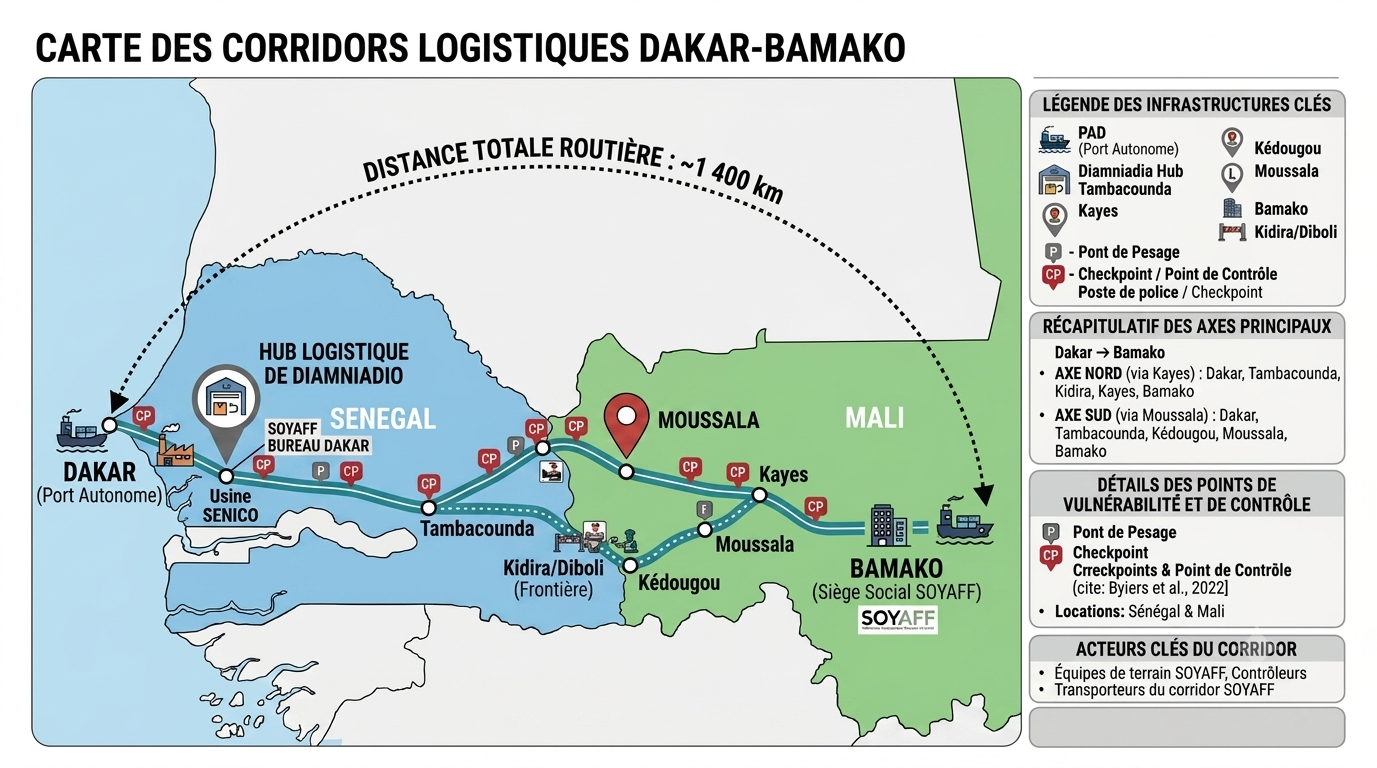
\includegraphics[width=0.95\textwidth]{figure_1_1_corridor}
  \caption{Corridor logistique Dakar--Bamako : axes routiers, ponts de
           pesage (Afrique Pesage S.A.) et checkpoints officiels et
           frontaliers (Kidira/Diboli pour l'axe nord, Moussala pour l'axe sud).}
  \source{Schéma illustratif de l'auteur, d'après Kébé et al.
          \cite{fix_kebeDiagnosticEntravesImportance2023}, Sigué \cite{sigueTransportRoutierMarchandises2017}, Byiers et Rosengren
          \cite{byiersActeursInteretsLong2022} et UEMOA/OPA \cite{uemoaOPA2017}}
  \label{fig:corridor_dakar_bamako}
\end{figure}

\subsection{Les acteurs clés de la chaîne logistique}
L'exploitation et la régulation de ce corridor font intervenir une multitude d'acteurs institutionnels et privés dont la coordination est essentielle. Au premier plan figurent les transporteurs routiers, segment composé de grands opérateurs logistiques mais également d'un tissu dense de Petites et Moyennes Entreprises (PME) nationales. Sur le plan régalien, l'administration des douanes sénégalaises et l'administration des douanes maliennes contrôlent la conformité des marchandises aux frontières. 

Les principaux points de passage frontaliers se concentrent au niveau de l'axe Kidira, du côté sénégalais, et de Diboli, du côté malien. Les Conseils nationaux des chargeurs, à savoir le Conseil Sénégalais des Chargeurs (COSEC) et le Conseil Malien des Transporteurs Routiers (CMTR), interviennent pour défendre les intérêts des opérateurs et faciliter les procédures. Bien que ces interactions s'inscrivent théoriquement dans les cadres communautaires de l'UEMOA et de la CEDEAO prônant la libre circulation des biens, l'application concrète de ces accords se heurte régulièrement à des freins administratifs et opérationnels majeurs.

Un acteur supplémentaire structure de façon déterminante le quotidien des transporteurs sur cet axe : le contrôle du gabarit, du poids et de la charge à l'essieu des poids lourds, encadré par le Règlement n\textsuperscript{o}14/2005/CM/UEMOA \cite{REGLEMENTNdeg142005}. Ce texte communautaire fixe des limites strictes que tout véhicule circulant sur le réseau routier des États membres doit respecter, qu'il s'agisse de la charge maximale autorisée à l'essieu (CMAE), du poids total autorisé en charge (PTAC) ou du poids total roulant autorisé (PTRA) pour les ensembles articulés. Au Sénégal, le contrôle de cette réglementation sur le réseau routier national a été délégué à un concessionnaire dédié, dont les stations fixes et mobiles sont notamment implantées sur les axes stratégiques de Mbour, Kaffrine, Tambacounda et Kidira, points de passage obligés pour les flux internationaux à destination du Mali. Pour les ensembles routiers internationaux tels que ceux exploités par SOYAFF, le respect simultané de ces deux contraintes (répartition correcte de la charge par essieu et plafond global du poids roulant) conditionne directement la fluidité du passage aux points de contrôle et constitue une source additionnelle de risque opérationnel (immobilisation, amende, délestage) en cas de non-conformité.

Pour rationaliser les contrôles routiers et accélérer le passage des corridors, l'État du Sénégal a adopté le décret n\textsuperscript{o}2021-1600 du 3 décembre 2021, complété par un arrêté interministériel instituant des brigades mixtes de contrôle routier (Gendarmerie, Police) et limitant en principe à trois le total des points de contrôle officiels par corridor national \cite{ControlesRoutiersAu2026}. Cette limitation théorique s'inscrit dans la lignée des recommandations communautaires de l'UEMOA, qui préconise également un plafond de trois postes de contrôle par corridor (au départ, au poste juxtaposé frontalier, et à destination). Dans la pratique cependant, la quantité de points de contrôle effectivement constatés sur le terrain dépasse régulièrement cette norme communautaire, comme le documentent les rapports périodiques de l'Observatoire des Pratiques Anormales (OPA) de l'UEMOA (cf. §1.1.3).

Une partie de ce dispositif de contrôle physique tend à être progressivement complétée, voire substituée, par des dispositifs de géolocalisation embarqués. D'après l'observation directe que nous avons conduite chez SOYAFF, une fraction significative de la flotte de camions de la société est équipée de balises de tracking GPS sur le territoire sénégalais, ce qui réduit dans certains cas la nécessité d'un contrôle physique systématique par les agents au profit d'un suivi à distance. Cette évolution, bien que partielle et non généralisée à l'ensemble du corridor, illustre une tendance plus large à la numérisation du contrôle logistique et renforce la pertinence d'une architecture capable d'exploiter de telles données de géolocalisation pour le suivi de flotte.

\subsection{Contraintes opérationnelles et vulnérabilités numériques}
L'efficacité du corridor Dakar--Bamako est lourdement grevée par la persistance de barrières non tarifaires, en dépit du cadre réglementaire théoriquement restrictif évoqué en §1.1.2. Si la norme communautaire de l'UEMOA et le décret sénégalais n\textsuperscript{o}2021-1600 fixent à trois le plafond de points de contrôle officiels par corridor, les rapports périodiques de l'OPA (initiative mise en place dès 2005 avec l'appui de l'USAID pour suivre la gouvernance routière dans l'espace communautaire) font régulièrement état d'un nombre de contrôles effectivement constatés sur le terrain bien supérieur à cette norme, ainsi que de prélèvements illicites persistants \cite{uemoaOPA2017}. Le corridor Dakar--Bamako figure parmi les axes où les temps de contrôle aux postes frontaliers sont les plus élevés de l'espace UEMOA, l'OPA ayant mesuré des temps moyens de l'ordre de 147 à 154 minutes selon le point de passage frontalier emprunté (Diboli ou Moussala) \cite{uemoaOPA2017}.

Cet écart entre le cadre réglementaire et la pratique observée engendre des retards systémiques et une inflation artificielle des coûts logistiques globaux. Les délais de transit s'avèrent de ce fait extrêmement variables, oscillant généralement entre 3 et 7 jours selon les conditions de circulation, les formalités douanières et les aléas administratifs. À ces frictions physiques s'ajoutent des enjeux de sécurité sur certains tronçons de l'itinéraire, obligeant les transporteurs à une vigilance accrue. 

Enfin, le corridor fait face à des vulnérabilités numériques notables. Conformément aux analyses de Cariolle \cite{cariolleInfrastructuresEconomieNumeriques2018}, les infrastructures de communication subissent des instabilités chroniques, allant des ruptures accidentelles de câbles sous-marins à une fracture numérique territoriale marquée entre les grands centres urbains et les zones frontalières enclavées.

\subsection{Les défis de gestion pour les PME de transport}
Pour les PME de transport routier, l'ensemble de ces contraintes se traduit par un manque aigu de visibilité sur la flotte en transit. Les difficultés de coordination asynchrone entre la plateforme de départ à Dakar et le siège décisionnel situé à Bamako nuisent à la productivité globale. En l’absence d'outils de suivi interconnectés, le pilotage en temps réel des camions devient impossible, laissant les gestionnaires désarmés face aux imprévus du corridor. C'est dans ce contexte que la société SOYAFF exerce son activité.

\section{La société SOYAFF : organisation et processus opérationnels}
\label{sec:soyaff_orga}

\subsection{Identification et activité de la société}
La société SOYAFF est une Petite et Moyenne Entreprise (PME) spécialisée dans la logistique et le commerce d'import-export, axée principalement sur la production, l'importation et la distribution de produits de première nécessité entre le Mali et le Sénégal. Pour soutenir cette activité transfrontalière et s'adapter aux configurations géographiques de la sous-région, la société dispose d'un siège social stratégique établi à Bamako (Mali) et d'une succursale opérationnelle implantée à Dakar (Sénégal). 

L'importance de son activité se reflète à travers la volumétrie substantielle enregistrée lors de notre travail de terrain : sur une fenêtre d'observation de 16 mois, SOYAFF a traité un total de 4~755 transactions, mobilisant 319 camions et générant 727 bons de chargement.

\begin{small}
\textit{L'utilisation des données opérationnelles de SOYAFF dans le cadre du présent travail a été formellement autorisée par la direction de la société, sous réserve d'anonymisation des informations financières et personnelles sensibles.}
\end{small}

\subsection{Structure organisationnelle et acteurs clés}
L'organisation humaine de SOYAFF repose sur une répartition géographique rigoureuse des rôles, nécessaire pour piloter un flux de marchandises s'étendant sur 1~400 kilomètres :
\begin{itemize}
    \item \textbf{À Bamako (Siège)} : Le chef logistique centralise les besoins du marché malien, planifie les grandes orientations de la flotte et attend les consolidations manuelles de données pour effectuer le reporting global destiné à la direction.
    \item \textbf{À Dakar (Succursale)} : L'équipe comprend un chef de bureau, un assistant principal et des agents de saisie chargés de consigner manuellement sur tableur les événements quotidiens liés à l'affrètement et au chargement des camions au départ du Port Autonome de Dakar.
    \item \textbf{Sur le corridor} : Une flotte de 45 chauffeurs actifs assure les liaisons de transport. La hiérarchie de validation des dépenses et des incidents suit un circuit strict allant du chauffeur vers l'assistant principal pour un premier visa, avant validation finale par le chef de bureau de Dakar.
\end{itemize}

\subsection{Cartographie des processus opérationnels quotidiens}
L'activité quotidienne génère un volume important de flux d'informations et de documents physiques. Le tableau \ref{tab:processus_soyaff} synthétise la nature, la fréquence et la volumétrie de ces processus que nous avons observés.

\begin{table}[htbp]
\centering
\caption{Synthèse des processus opérationnels et volumétries chez SOYAFF}
\label{tab:processus_soyaff}
\begin{tabular}{|>{\raggedright\arraybackslash}p{4.3cm}|>{\raggedright\arraybackslash}p{2.4cm}|>{\raggedright\arraybackslash}p{2.6cm}|>{\raggedright\arraybackslash}p{3.4cm}|}
\hline
\textbf{Processus} & \textbf{Fréquence} & \textbf{Volume estimé} & \textbf{Support actuel} \\ \hline
Plans de chargement camions & Quotidien & 5 à 10 / jour & Fiches papier + Excel \\ \hline
Gestion des contraventions & Variable & 2 à 8 / semaine & Excel + reçus papier \\ \hline
Rations chauffeurs (séjour > 5j) & Hebdomadaire & $\sim$15 / semaine & Fiches \texttt{AUT-DEP} papier \\ \hline
Primes de liaison & À chaque liaison & $\sim$25 / mois & Excel + reçus \\ \hline
Frais mécaniques et pièces & Variable & $\sim$30 / mois & Factures papier + Excel \\ \hline
Récapitulatif journalier & Quotidien & 1 / jour & Fichier Excel \\ \hline
Récapitulatif mensuel & Mensuel & 1 / mois & Excel consolidé \\ \hline
\end{tabular}
\end{table}

\subsection{Outils technologiques en usage}
Le système d’information actuel de la société SOYAFF se caractérise par une absence totale de base de données centralisée ou de progiciel de gestion intégré (ERP). Les outils se limitent à l'utilisation de fichiers de tableurs décentralisés, principalement dénommés \texttt{RECAP-JOURNALIERE} et \texttt{RECAP-MENSUEL}. Les autorisations de dépenses et le suivi des frais s'appuient sur des fiches physiques au format papier, appelées fiches \texttt{AUT-DEP} (Autorisation de Dépense). Les flux de communication formels s'effectuent par courrier électronique, tandis que la coordination informelle et instantanée des urgences sur le corridor (pannes, blocages aux checkpoints) repose sur l'application grand public WhatsApp. Une application mobile tierce, \texttt{kiri.app}, est aussi en usage, mais son périmètre se limite strictement à la conformité administrative (collecte des pièces signées par les représentants logistiques) : elle ne propose aucun module de suivi de caisse, de tableau de bord ou d'analyse décisionnelle.

\section{Diagnostic du système d'information existant}
\label{sec:diagnostic_si}

\subsection{Flux d'information actuel et rupture de saisie}
Le parcours d'une donnée opérationnelle au sein de SOYAFF met en lumière une rupture flagrante dans la chaîne de traitement de l'information. Lorsqu'un camion est chargé ou qu'un frais est engagé à Dakar, l'agent de saisie local consigne l'information dans son fichier Excel récapitulatif. En fin de journée, ce document \texttt{RECAP-JOURNALIERE} est transmis par e-mail ou via WhatsApp au siège à Bamako. 

À la réception, le chef logistique de Bamako doit ouvrir le fichier et procéder à une \textbf{ressaisie manuelle intégrale}, ligne par ligne, de l'ensemble des transactions dans sa propre base de données locale afin de pouvoir calculer les agrégats de performance. Cette double saisie systématique crée une zone de vulnérabilité majeure : toute erreur ou besoin de clarification impose de longs échanges et des allers-retours correctifs asynchrones par téléphone ou messagerie entre Dakar et Bamako.

\subsection{Analyse ancrée : Les contraintes macro du corridor face au micro-système}
Pour comprendre la fragilité du système d'information de SOYAFF, il faut le confronter aux réalités du corridor routier Dakar–Bamako. Selon les données de l'OPA, ce corridor long de près de 1~400 km subit une moyenne critique de \textbf{31,47 contrôles routiers par voyage} (soit environ 2,13 points de contrôle pour 100 km), générant des perceptions illicites moyennes de 43~078 F~CFA par trajet pour un camion pourtant en règle \cite{fix_kebeDiagnosticEntravesImportance2023}. Ce chiffre confirme, à une échelle plus précise, l'écart déjà constaté en §1.1.3 entre le plafond réglementaire de trois points de contrôle par corridor et la réalité du terrain.

De plus, l'axe détient un temps d'attente cumulé élevé aux points de passage frontaliers, atteignant une moyenne de \textbf{316 minutes de stagnation} par voyage du fait de la lenteur des formalités douanières administratives \cite{sigueTransportRoutierMarchandises2017}. En l'absence d'un système d'information interconnecté, ces événements imprévisibles (perceptions informelles sans reçu officiel, immobilisations prolongées aux gares de rupture de charge) sont gérés de manière totalement opaque par des messages WhatsApp volatils, empêchant la PME d'anticiper la rotation théorique de ses camions, estimée en moyenne à 14 jours sur cet axe \cite{sigueTransportRoutierMarchandises2017}.

\subsection{Typologie des limites observées}
L'analyse critique du système actuel permet de classifier ses faiblesses structurelles en quatre catégories distinctes :
\begin{enumerate}
    \item \textbf{Limites opérationnelles} : La double saisie systématique s'avère extrêmement chronophage, consommant en moyenne 2 à 3 heures de travail quotidien pour le seul chef logistique à Bamako. Ce mode de fonctionnement asynchrone induit une latence d'information de 24 à 48 heures, empêchant toute exploitation immédiate des données opérationnelles du jour J. Enfin, le transfert manuel de fichiers isolés par e-mail expose l'entreprise à des risques élevés de perte de données ou de désynchronisation de versions.
    \item \textbf{Limites qualitatives} : La manipulation humaine répétée de milliers de lignes engendre inévitablement des erreurs de saisie (inversion de dates, fautes de frappe sur les immatriculations ou les montants), des doublons, des omissions et des ruptures fréquentes de formules de calcul au sein des tableurs Excel lors des consolidations mensuelles.
    \item \textbf{Limites décisionnelles} : La direction ne dispose d'aucun tableau de bord mis à jour en temps réel. Il est impossible d'extraire instantanément des analyses avancées, telles que la dérive des coûts de carburant par camion ou les tendances de performance de la flotte face au harcèlement routier. Les décisions managériales sont ainsi guidées par l'intuition et l'expérience empirique plutôt que par des indicateurs factuels fiables.
    \item \textbf{Limites stratégiques} : L'absence d’historique centralisé, sécurisé et structuré au-delà du mois courant bloque toute tentative de planification ou d'analyse prédictive à moyen terme. Ce système bloque la croissance : si la flotte de camions venait à s'agrandir, la structure administrative actuelle s'effondrerait sous le poids des ressaisies manuelles et de l'asynchronisme.
\end{enumerate}

\subsection{Conséquences financières et organisationnelles}
Les impacts de cette dette opérationnelle sont multiples et se déclinent sur trois plans complémentaires.

Sur le plan financier, le coût caché lié au temps passé par des cadres qualifiés à ressaisir des lignes Excel représente une perte économique quantifiable à l'échelle de l'exercice annuel. En prenant pour base les 2 à 3 heures quotidiennes consacrées à la double saisie par le chef logistique de Bamako (cf. §1.3.3), et en valorisant ce temps au coût horaire chargé d'un cadre logistique dans la sous-région, la perte annuelle directement imputable à cette seule tâche redondante peut être estimée à plusieurs centaines d'heures de travail qualifié, soit l'équivalent de plusieurs mois-homme par an. À cela s'ajoute un coût indirect, plus difficile à quantifier mais tout aussi réel : la non-détection en temps réel des taxes informelles (43~078 F~CFA en moyenne par trajet selon les données de l'OPA, cf. §1.3.2) et des failles logistiques grève directement la rentabilité de l'entreprise, sans que la direction dispose des moyens de les anticiper ou de les contester.

Sur le plan organisationnel, la lourdeur des processus engendre une frustration partagée par les équipes et crée une dépendance critique vis-à-vis d'individus clés, détenteurs exclusifs des fichiers tableurs. Cette concentration du savoir opérationnel constitue un facteur de risque significatif : l'absence ou le départ d'un agent de saisie expérimenté peut paralyser temporairement la chaîne de remontée d'information. Face à un corridor en voie de modernisation et d'intégration régionale accélérée (ZLECAf, guichets uniques portuaires), l'absence de transformation numérique expose SOYAFF à un risque majeur de perte de compétitivité face à des concurrents plus agiles.

Enfin, sur le plan stratégique, cette situation prive la direction de SOYAFF d'un levier essentiel de pilotage : sans visibilité fiable sur les coûts réels par trajet, par camion ou par chauffeur, toute décision d'investissement (renouvellement de flotte, ouverture de nouvelles lignes, négociation tarifaire) repose sur des estimations approximatives plutôt que sur des données consolidées.

\section{Synthèse du diagnostic et positionnement du projet}
\label{sec:synthese_diagnostic}

L'analyse conduite dans ce chapitre met en évidence une situation paradoxale, déjà identifiée à l'échelle macro-économique en introduction : alors que le corridor Dakar--Bamako constitue un axe stratégique majeur pour l'économie malienne, et que SOYAFF y occupe une position d'acteur logistique établi traitant plusieurs milliers de transactions sur 16 mois, son système d'information repose encore intégralement sur des outils bureautiques non interconnectés. SOYAFF n'est pas un cas à part : l'entreprise évolue dans un secteur précis, sur un corridor bien déterminé, ce qui la rend représentative des PME d'import-export opérant sur des corridors comparables en Afrique de l'Ouest, où la digitalisation reste largement à faire.

Ce diagnostic oriente la suite du travail. Les dysfonctionnements observés ne viennent pas d'un manque de volonté ou de compétence des équipes, mais d'un outillage inadapté à leur contexte : connexion intermittente, budget serré, deux sites distants de 1~400 kilomètres. Toute solution devra composer avec ces contraintes. La typologie des limites (\S\ref{sec:diagnostic_si}) servira de grille pour structurer les exigences du système (section~\ref{chap:besoins}). Enfin, la nature des données traitées (montants, identités des chauffeurs) fait de la souveraineté une contrainte de conception, et non une option. C'est elle qui justifie une architecture combinant une IA générative cloud et une IA auto-hébergée.

Une solution générique ne suffit donc pas pour SOYAFF. L'entreprise n'est pas prête à investir lourdement dans sa digitalisation, quitte à rester sur Excel ; elle travaille avec une connexion instable ; et son chef logistique refuse que les données partent chez un tiers. L'architecture doit répondre à ces trois réalités.

\section{Objectifs de l'étude}
\label{sec:objectifs}

\textbf{Objectif général (OG).} Concevoir, déployer et évaluer scientifiquement une architecture logicielle hybride et réplicable pour la digitalisation des PME d'import-export en Afrique subsaharienne, en prenant SOYAFF comme cas de validation principal.

\textbf{Objectifs spécifiques (OS).} Pour y parvenir, nous nous sommes fixé les objectifs suivants :
\begin{itemize}
    \item[\textbf{OS1}] \textbf{Documenter} l'état de l'art sur la digitalisation des PME africaines, les architectures ETL, les systèmes RAG et la souveraineté numérique.
    \item[\textbf{OS2}] \textbf{Caractériser} le domaine des PME d'import-export ouest-africaines pour en dégager les invariants et les points de variation.
    \item[\textbf{OS3}] \textbf{Spécifier} l'architecture selon le modèle C4, en justifiant chaque choix par un \textit{Architecture Decision Record} (ADR).
    \item[\textbf{OS4}] \textbf{Mettre en œuvre, déployer et exploiter} la plateforme en production sur le cas SOYAFF.
    \item[\textbf{OS5}] \textbf{Mener} un benchmark comparant le RAG cloud et le RAG local sur 30 questions métier représentatives, puis \textbf{mesurer} l'impact métier et le coût réel de la solution (gain horaire, taux d'erreur, coût mensuel).
    \item[\textbf{OS6}] \textbf{Étudier} l'adoption utilisateur avec le questionnaire \textit{System Usability Scale} (SUS) et des entretiens semi-directifs.
    \item[\textbf{OS7}] \textbf{Analyser} la généralisation de l'architecture avec l'approche des lignes de produits logiciels (\textit{Software Product Lines}), pour distinguer ce qui reste stable de ce qui doit être reconfiguré d'une PME à l'autre.
    \item[\textbf{OS8}] \textbf{Formaliser} un référentiel d'architecture réplicable, utile à la recherche comme à d'autres projets du même type.
\end{itemize}

\section{Méthodologie de recherche}
\label{sec:methodologie}

Pour mener à bien ce projet, nous adoptons une approche entre ingénierie logicielle et évaluation scientifique. Sur le plan de l'ingénierie, nous appliquons une démarche hybride agile, combinant des cycles itératifs avec une formalisation systématique des choix architecturaux via des ADR (\textit{Architecture Decision Records}). La modélisation s'appuie sur le framework C4 (Context, Container, Component, Code), enrichi par les diagrammes UML pertinents. En outre, pour le développement de nouvelles fonctionnalités, nous adoptons une démarche inspirée de Scrum : chaque fonctionnalité fait l'objet d'un ticket Jira classé par priorité dans un sprint, et une branche Git dédiée est créée pour chaque ticket. Le code est hébergé et déployé sur GitLab, où chaque \textit{push} sur la branche principale déclenche automatiquement le pipeline de déploiement (voir section~\ref{chap:devops}).

Côté scientifique, l'évaluation repose sur trois angles. D'abord un benchmark qui compare les deux systèmes RAG sur la latence, l'exactitude et le taux d'hallucination. Ensuite une étude avant/après digitalisation pour chiffrer les gains opérationnels. Et pour l'adoption utilisateur, nous nous appuyons sur le questionnaire \textit{System Usability Scale} (SUS) \cite{brookeSUSAQuickDirty1996} et sur des entretiens semi-directifs.

Le benchmark comparatif constitue le cœur de l'évaluation scientifique. Il repose sur un corpus de 30 questions métier, six par catégorie fonctionnelle : suivi de flotte, gestion financière, analyse des incidents, conformité documentaire et aide à la décision stratégique. Chaque question est aussi classée selon le type de réponse attendue : T1 pour un chiffre ou un fait vérifiable par une requête SQL (15 questions), T2 pour une liste (10 questions), T3 pour une analyse jugée sur grille (5 questions). Les deux systèmes sont interrogés trois fois par question sur le serveur de production. Nous mesurons la latence (P50, P95, P99), l'exactitude par comparaison à une vérité-terrain fixée avant toute exécution, le taux d'hallucination, le coût par requête et le niveau de souveraineté des données. Ce protocole s'appuie sur les travaux de Lewis et al. \cite{lewisRetrievalaugmentedGenerationKnowledgeintensive2020} sur la génération augmentée par récupération et sur le cadre d'évaluation de Gao et al. \cite{gaoRetrievalAugmentedGenerationLarge2024}.

Afin d'éprouver la capacité de généralisation de la solution (hypothèse H4), l'analyse s'inspirera de l'approche des lignes de produits logiciels (\textit{Software Product Lines}) pour dissocier le noyau stable de l'architecture de ses points de variation, sans recourir à une étude empirique multi-cas dont la réalisation dépasse le cadre temporel de ce mémoire. Cette piste empirique est identifiée comme une perspective de recherche future. L'ensemble de ces travaux respecte l'éthique de la recherche : nous anonymisons les données réelles, nous recueillons le consentement des parties prenantes, et l'architecture respecte la loi 2008-12 du Sénégal sur la protection des données à caractère personnel.